%!TEX root = ../../main.tex

\chapter{Konfigurationsmanagement}
Alle Dateien werden über den Versionsverwaltungsdienst GitHub versioniert und unter den Projektteilnehmern ausgetauscht.\\
Das Repository befindet sich \href{https://github.com/LucRome/SWE_Semester4}{hier}.\\

Zur Gestaltung des Repositorys sind folgende Regeln zu beachten:
Jedes Themengebiet (Frontend, Backend und Dokumentation) hat seinen eigenen Branch.
Der Zugriff auf diesen Branch kann nochmals intern eingeschränkt werden. Dies wird von den einzelnen Arbeitsteams aufgabenbezogen festgelegt. \\
Ein Commit auf den Master-Branch kann erst ausgeführt werden, wenn alle Punkte der Definition Of Done (siehe \ref{fib:DOD}) abgearbeitet sind. \\
Dies beinhaltet, dass der Code getestet ist, den Codierungsrichtlinien in Kapitel \ref{sec:Chap2} entspricht und von mindestens einer anderen Person des Developmentteams abgenommen wurde. \\

\begin{figure}[H]
\centering
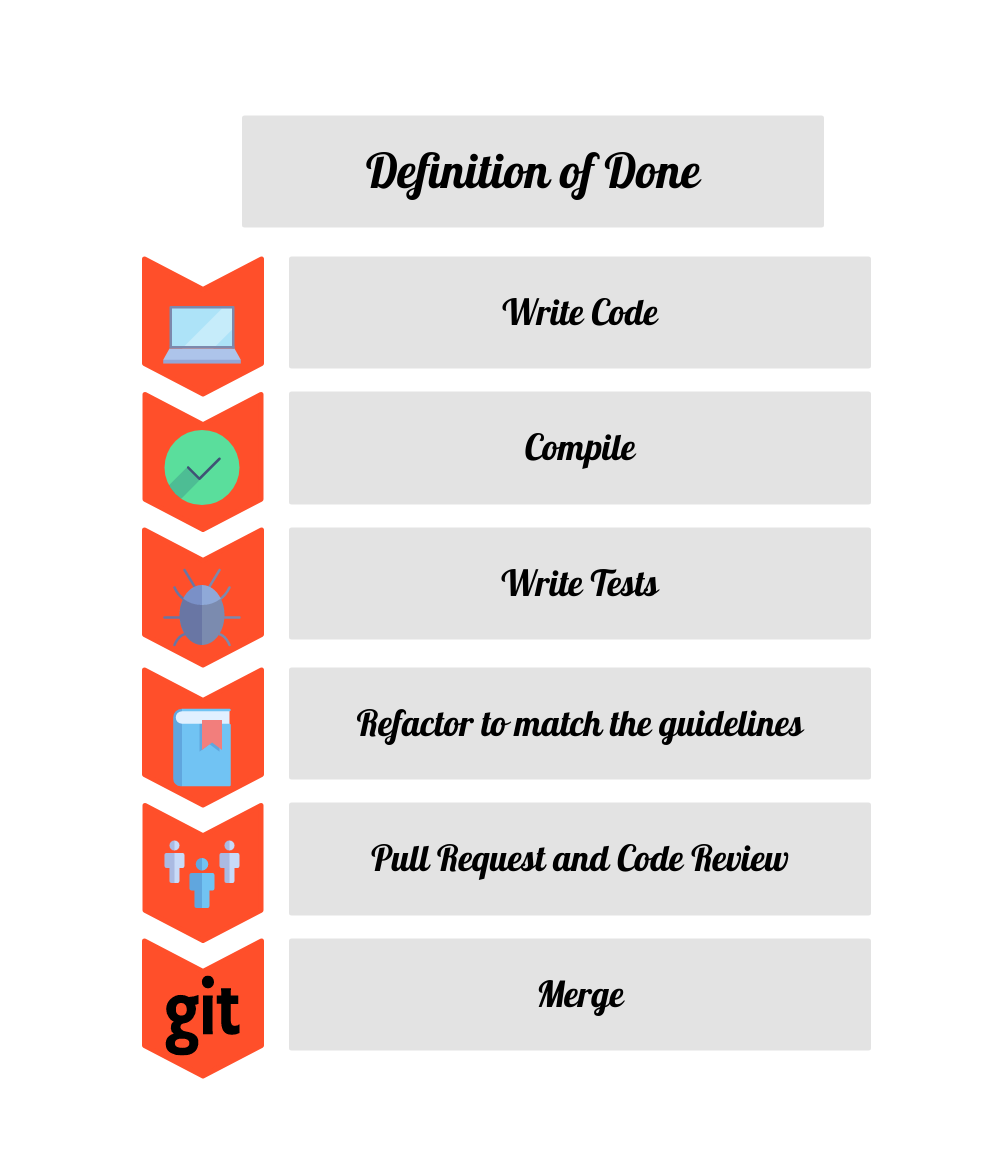
\includegraphics[height=.6\textwidth]{definition_of_done.png}
\caption{Definition of Done}
\label{fib:DOD}
\end{figure}

Jeder Commit wird mit einer Zusammenfassung und einer tiefer gehenden Beschreibung versehen. \\
Die Zusammenfassung enthält dabei eine kurze Beschreibung des geänderten Merkmals. \\
Die Beschreibung geht dann genauer auf das geänderte Merkmal ein. \\

Des Weiteren befinden sich im Repository noch ein Kanban-Board, ein Wiki und eine Issue-Liste.\\
Das Kanban-Board wird zur Organisation des aktuellen Sprints eingesetzt. Dafür werden alle Tasks des aktuellen Sprints gesammelt. Diese werden dann an die Arbeitsgruppen verteilt und von diesen Bearbeitet. Ist ein Task aus Sicht der Arbeitsgruppe fertiggestellt, verschieben sie diesen in die Review-Leiste. Dies signalisiert den anderen Gruppen, dass die Arbeit des Teams überprüft werden kann. Wird der Task als erledigt angesehen, kann er in die Done-Leiste geschoben werden.\\

Im Wiki können alle Informationen die für alle Teams wichtig sind gesammelt werden. Dabei handelt es sich vor allem um Informationen, die schnell und immer verfügbar sein sollten.\\

In der Issue-Liste können dann neben den aktuell laufenden Tasks auch während der Entwicklung auftauchende Bugs aufgenommen werden.

